\section{Data acquisition and preprocessing }
\label{section:Data_acquisition_and_preprocessing}
%%%%%%%%%%%%%%%%%%%%%%%%%%%%%%%%%%%%%%%%%%%%%%%%%%%%%
In this section, the numerically generated dataset of full wavefield images is presented, then, the applied data preprocessing techniques is illustrated. 
%%%%%%%%%%%%%%%%%%%%%%%%%%%%%%%%%%%%%%%%%%%%%%%%%%%%%
\subsection{Dataset}
%%%%%%%%%%%%%%%%%%%%%%%%%%%%%%%%%%%%%%%%%%%%%%%%%%%%%
In our previous work, we have explained the procedure of generating a large dataset of 475 cases of a full wavefield of propagating Lamb waves in a plate made of carbon fibre reinforced plastic (CFRP). 
For further explanation, the reader is advised to refer to our previous work titled (Full Wavefield Processing by Using FCN for Delamination Detection).
As mentioned in our previous work, we have applied the time-domain spectral element method in order to simulate Lamb wave interaction with delamination~\cite{Kudela2020}. 
The dataset computation took about 3 months, in which the parallel code of the spectral element method was implemented to run in Tesla K20X GPU card.
The method of splitting nodes between appropriate spectral elements was used to model every single delamination in all cases.
In our work, the composite laminate was assumed to be made of eight layers of a total thickness of \(3.9\) mm.
As shown in Fig.~\ref{fig:plate_setup} the delamination was modelled between the third and the fourth layer.


It should be noted that Fig.~\ref{fig:plate_setup} shows an exaggerated cross-section through the delamination. 
Zero-volume delamination was assumed in the model. 
Delamination spatial location was selected randomly so that the interaction of guided waves with delamination is different for each case.
It includes cases when delamination is located at the edge of the plate which is the most difficult to identify by signal processing methods.
Additionally, the size of the delamination was randomly simulated by selecting the ellipse minor and major axis from the interval 10--40 mm.
Also, the angle between the delamination major axis and the horizontal axis was randomly selected.

\begin{figure}
	\centering
	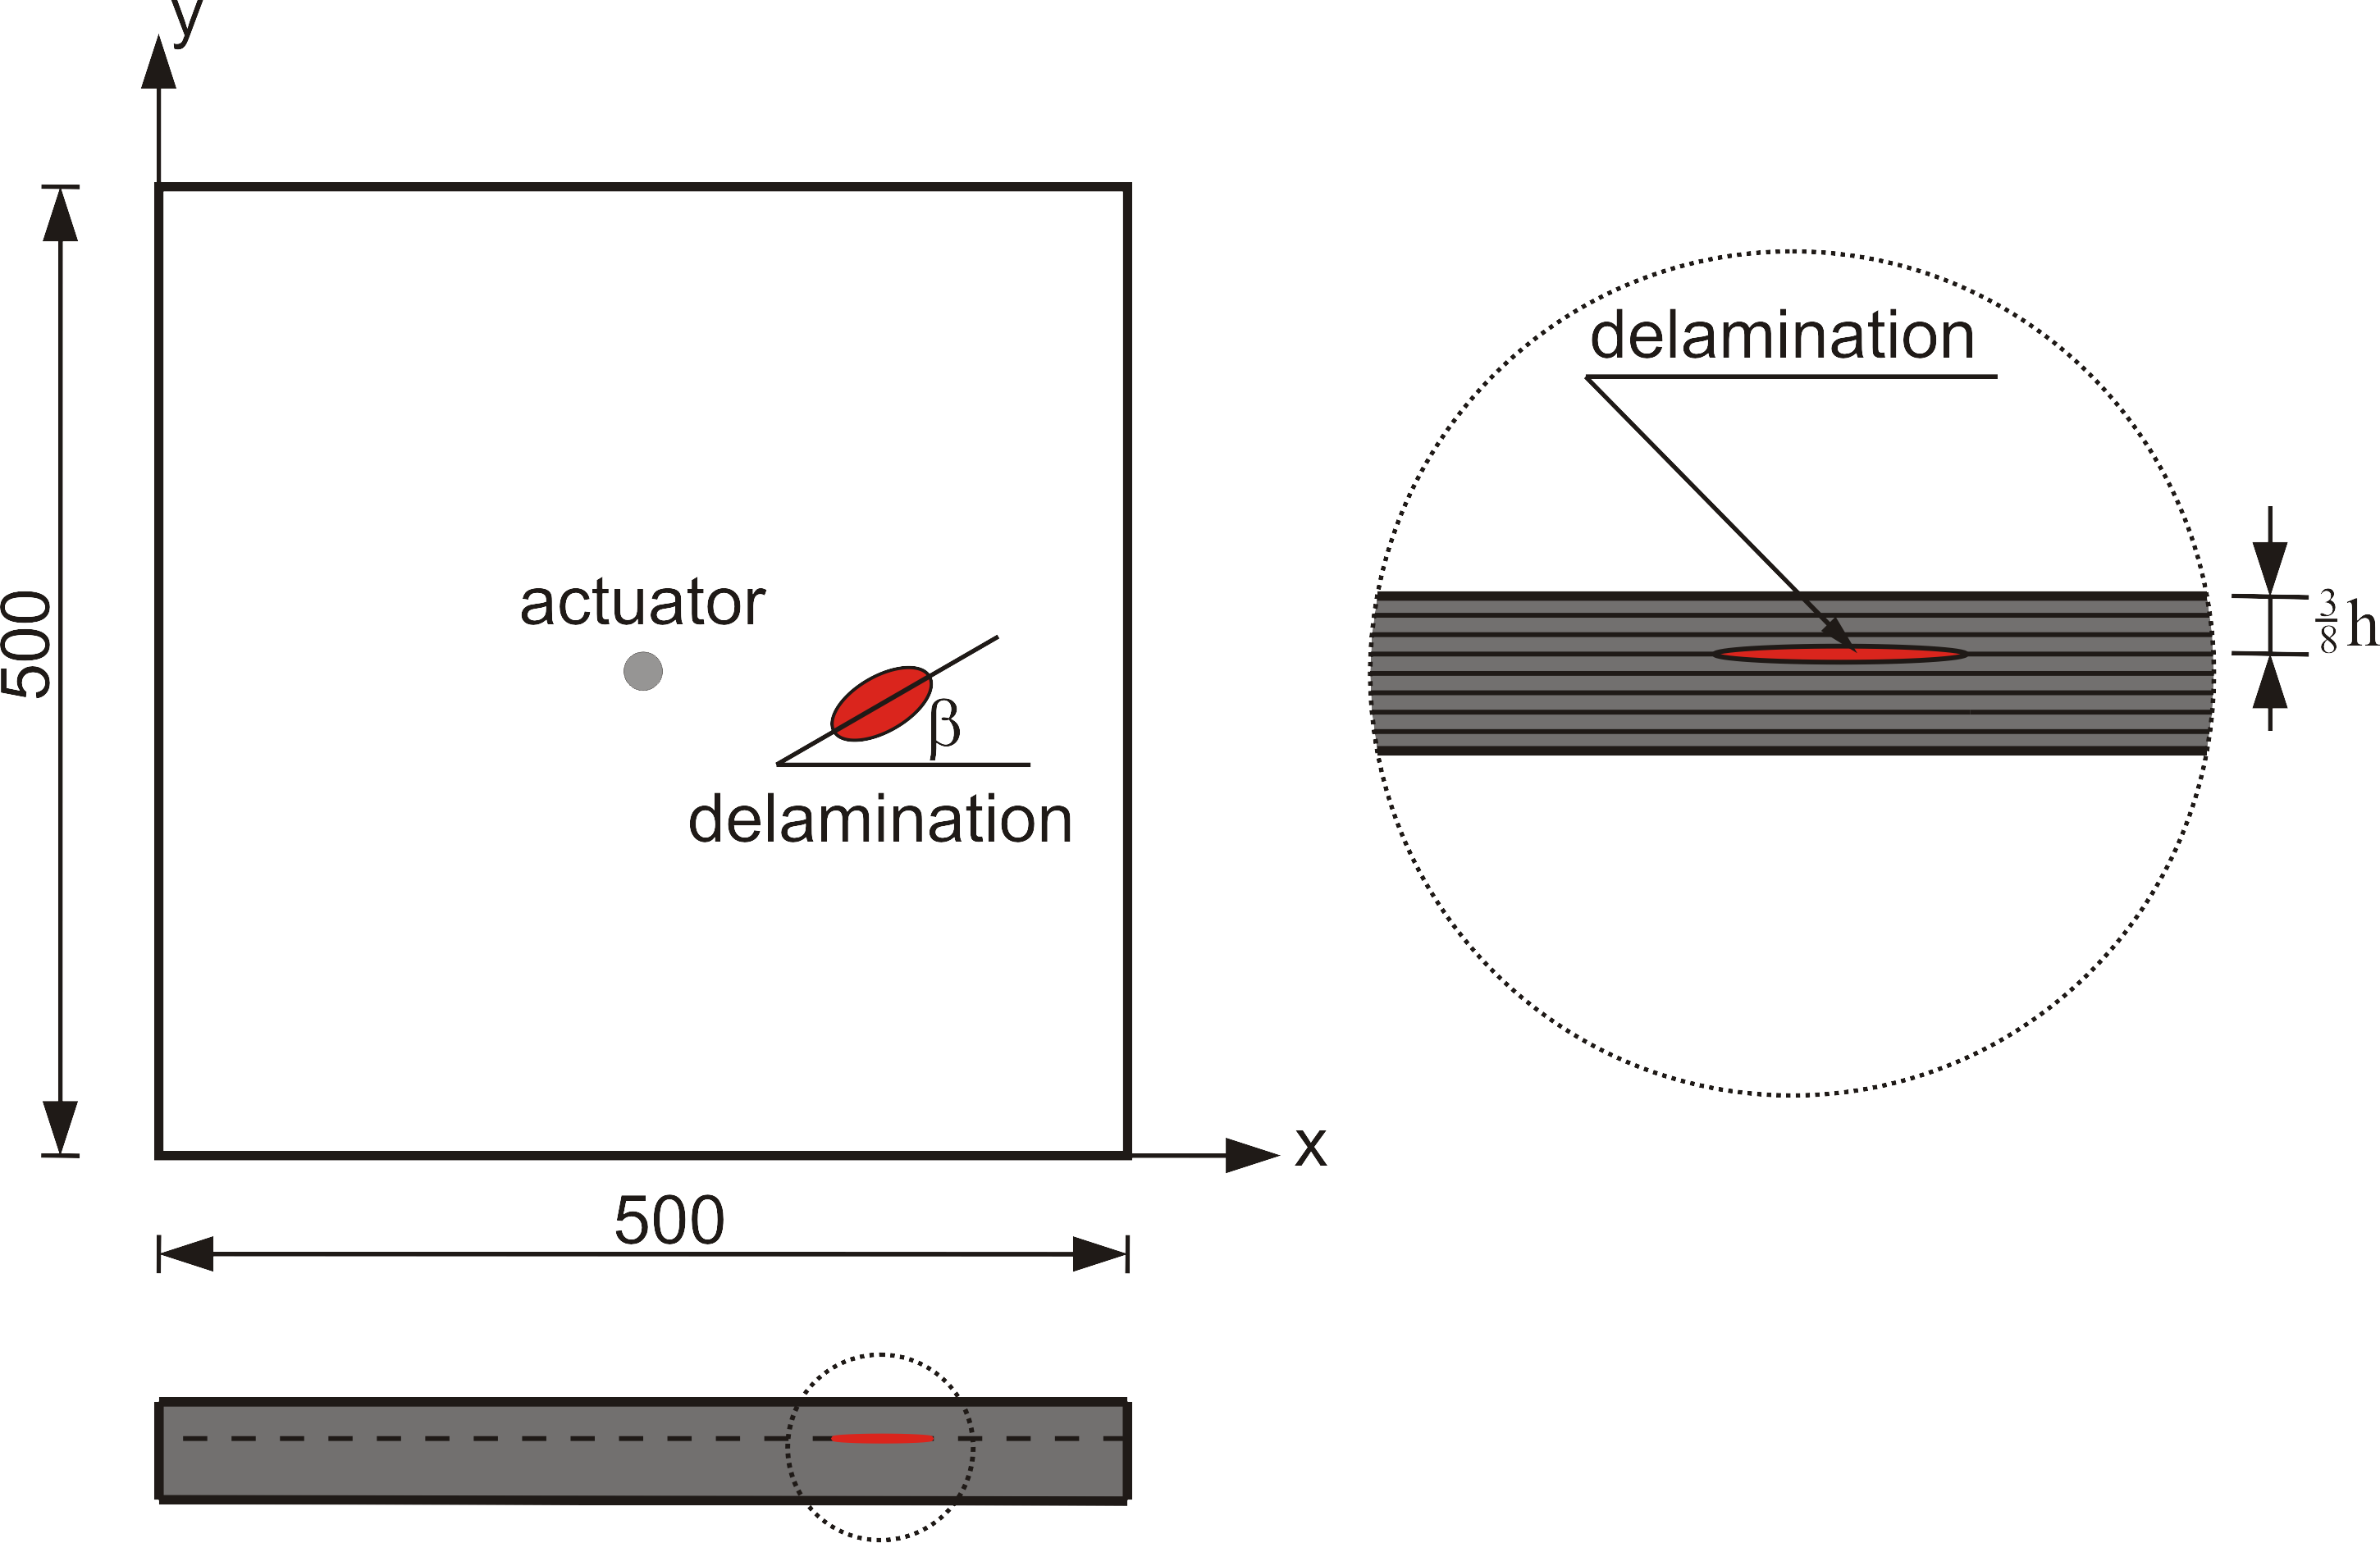
\includegraphics[scale=0.8]{plate_delam_arrangement_MSSP.png}
	\caption{Setup for computing Lamb wave interactions with delamination.}
	\label{fig:plate_setup}
\end{figure}	
	
Guided waves were excited at the plate centre by applying equivalent piezoelectric forces.
The excitation signal had a form of sinusoid modulated by Hann window. 
It was assumed that the carrier frequency is 50 kHz and the modulation frequency is 10 kHz.

The output from the top and bottom surfaces of the plate in the form of particle velocities at the nodes of spectral elements were interpolated on the uniform grid of 500\(\times\)500 points by using shape functions of elements (see~\cite{Kudela2020} for more details).
It essentially resembles measurements acquired by SLDV in the transverse direction (perpendicular to the plate surface). 
The root mean square (RMS) according to Eq.~(\ref{eq:rms}) is applied to the wavefield.
Based on the image analysis, the shape of the delamination can be easier to discern for the top case.
However, the methodology presented in this paper was applied to the more difficult case i.e. wavefield registered at the bottom surface of the plate.

%\begin{figure} [h!]
%	\centering
%	\begin{subfigure}[b]{0.32\textwidth}
%		\centering
%		\includegraphics[scale=1]{96_flat_shell_Vz_1_500x500top.png}
%		\caption{\(t=0.141\) ms}
%		\label{fig:frame96top}
%	\end{subfigure}
%	\hfill
%	\begin{subfigure}[b]{0.32\textwidth}
%		\centering
%		\includegraphics[scale=1]{128_flat_shell_Vz_1_500x500top.png}
%		\caption{\(t=0.188\) ms}
%		\label{fig:frame128top}
%	\end{subfigure}
%	\hfill
%	\begin{subfigure}[b]{0.32\textwidth}
%		\centering
%		\includegraphics[scale=1]{164_flat_shell_Vz_1_500x500top.png}
%		\caption{\(t=0.240\) ms}
%		\label{fig:frame164top}
%	\end{subfigure}	
%	\hfill
%	\begin{subfigure}[b]{0.32\textwidth}
%		\centering
%		\includegraphics[scale=1]{96_flat_shell_Vz_1_500x500bottom.png}
%		\caption{\(t=0.141\) ms}
%		\label{fig:frame96bottom}
%	\end{subfigure}
%	\hfill
%	\begin{subfigure}[b]{0.32\textwidth}
%		\centering
%		\includegraphics[scale=1]{128_flat_shell_Vz_1_500x500bottom.png}
%		\caption{\(t=0.188\) ms}
%		\label{fig:frame128bottom}
%	\end{subfigure}
%	\hfill
%	\begin{subfigure}[b]{0.32\textwidth}
%		\centering
%		\includegraphics[scale=1]{164_flat_shell_Vz_1_500x500bottom.png}
%		\caption{\(t=0.240\) ms}
%		\label{fig:frame164bottom}
%	\end{subfigure}
%
%	\caption{Full wavefield at the top surface (a)--(c) and the bottom surface (d)--(f), respectively, at selected time instances showing the interaction of guided waves with delamination.}
%	\label{fig:wavefield}
%\end{figure} 

\begin{figure} [h!]
	\centering
	\begin{subfigure}[b]{0.47\textwidth}
		\centering
		\includegraphics[scale=.29]{RMS_flat_shell_Vz_27_500x500top.png}
		\caption{top}
		\label{fig:rmstop}
	\end{subfigure}
	\hfill
	\begin{subfigure}[b]{0.47\textwidth}
		\centering
		\includegraphics[scale=.29]{RMS_flat_shell_Vz_27_500x500bottom.png}
		\caption{bottom}
		\label{fig:rmsbottom}
	\end{subfigure}
	\caption{RMS of the full wavefield from the top surface of the plate (a) and the bottom surface of the plate (b).}
\label{fig:rms}
\end{figure} 